\section{Bộ dữ liệu và phương pháp thu thập}
    
    \subsection{Nguồn và quy trình thu thập}
    \texttt{core/Get\_frame.py} gửi yêu cầu đến đường dẫn \texttt{render/ImageHandler.ashx} của nguồn camera giao thông TP.HCM. Yêu cầu chứa định danh camera và tham số thời gian, kèm User-Agent, Referer, thời gian chờ 10 giây. Dữ liệu trả về được chuyển thành mảng NumPy và giải mã bằng \texttt{cv2.imdecode()}.

    \texttt{get\_data.py} thực hiện quy trình sau:
    \begin{enumerate}
        \item Lấy ảnh từ camera được chọn, mặc định là Camera 1.
        \item Ghi nhận thời gian máy nhận ảnh trước khi chạy nhận diện.
        \item So sánh \texttt{frame.tobytes()} với ảnh ngay trước đó. Nếu giống hoàn toàn, không tạo thêm mẫu nhận diện.
        \item Chạy YOLO trên ảnh mới, đếm phương tiện và tính WTI.
        \item Ghi kết quả thành CSV theo lô mỗi 5 mẫu; ghi phần còn lại trong khối \texttt{finally} khi thoát bình thường hoặc có ngoại lệ đi qua khối này.
    \end{enumerate}
    Collector mặc định chạy tối đa 86.400 giây, tương đương 24 giờ. Tên đầu ra đã tồn tại bị từ chối nhằm giữ nguyên đợt thu trước. Dữ liệu thực tế có khoảng cách mẫu trung vị 12 giây; đây là nhịp quan sát đo được, không phải bảo đảm rằng camera nguồn phát ảnh mới chính xác mỗi 12 giây.

    Việc so sánh bytes chỉ phát hiện ảnh lặp hoàn toàn liên tiếp. Nó không xác minh độ mới của ảnh phía camera, không nhận biết mọi trường hợp ảnh gần giống và không thay thế được kiểm tra chất lượng nhận diện. Timestamp trong CSV không có thông tin múi giờ; hệ thống xử lý chúng theo quy ước giờ địa phương Việt Nam. Do CSV cũ không lưu phiên bản collector, không thể khẳng định mọi dòng lịch sử đều được tạo bằng chính phiên bản mã hiện tại.

    \subsection{Quy mô và cấu trúc}
    Hai CSV chứa tổng cộng 14.109 bản ghi và 9 cột, tương ứng hai đợt quan sát gần 24 giờ, cách nhau khoảng một tuần. Trong thiết kế huấn luyện, \texttt{data1} dùng cho fit/validation và refit; \texttt{data2} dùng để đánh giá sau khi chọn cách biểu diễn mục tiêu.

    \begin{table}[htbp]
        \centering
        \caption{Thuộc tính của hai tập dữ liệu}
        \vspace{0.2cm}
        \begin{tabular}{|p{7cm}|p{4cm}|p{4cm}|}
            \hline
            \textbf{Thuộc tính} & \textbf{data1} & \textbf{data2} \\
            \hline
            Số bản ghi gốc & 7.044 & 7.065 \\
            \hline
            Bắt đầu CSV & 21/09/2026 17:41:40 & 28/09/2026 22:39:52 \\
            \hline
            Kết thúc CSV & 22/09/2026 17:41:32 & 29/09/2026 22:39:43 \\
            \hline
            Số mốc phút sau loại hai biên không đầy đủ & 1.439 & 1.439 \\
            \hline
            Phút hoàn toàn không có mẫu & 2 & 3 \\
            \hline
            Phút chỉ có 1–2 mẫu & 4 & 6 \\
            \hline
            Khoảng cách mẫu trung vị & 12 giây & 12 giây \\
            \hline
            Khoảng cách mẫu lớn nhất & 147 giây & 170 giây \\
            \hline
            Cửa sổ đủ lịch sử và đủ 60 mục tiêu & 1.098 & 956 \\
            \hline
        \end{tabular}
    \end{table}

    Một “cửa sổ” hay forecast origin là thời điểm phát dự báo có đủ đầu vào và đầu ra tương lai để đánh giá. Các cửa sổ liên tiếp dùng chung phần lớn lịch sử và mục tiêu; 956 origin không tương đương 956 tình huống giao thông độc lập.

    \begin{table}[htbp]
        \centering
        \caption{Ý nghĩa các cột trong tập dữ liệu}
        \vspace{0.2cm}
        \begin{tabular}{|p{4cm}|p{12cm}|}
            \hline
            \textbf{Cột CSV} & \textbf{Ý nghĩa và vai trò} \\
            \hline
            \texttt{timestamp} & Thời điểm bản ghi, định dạng YYYY-MM-DD HH:MM:SS \\
            \hline
            \texttt{person} & Số đối tượng người; không dùng làm đặc trưng dự báo hiện tại \\
            \hline
            \texttt{car, motorbike, bus, truck} & Số phát hiện của bốn loại phương tiện trong ảnh \\
            \hline
            \texttt{total} & Tổng số phát hiện của bốn loại xe \\
            \hline
            \texttt{WTI} & Điểm trọng số phương tiện; cơ sở tạo target theo phút \\
            \hline
            % \texttt{WTI\_norm} & WTI nhân hệ số logarit theo tổng số xe; không dùng trong model hiện tại \\
            % \hline
        \end{tabular}
    \end{table}

    \subsection{Phân bố quan sát}
    Các thống kê dưới đây được tính lại trực tiếp từ từng dòng CSV, trước khi tổng hợp theo phút. Độ lệch chuẩn trong bảng là độ lệch chuẩn mẫu.

    \begin{table}[htbp]
        \centering
        \caption{Thống kê phân bố quan sát}
        \vspace{0.2cm}
        \begin{tabular}{|p{6cm}|p{4cm}|p{4cm}|}
            \hline
            \textbf{Thống kê} & \textbf{data1} & \textbf{data2} \\
            \hline
            Số xe trung bình/ảnh & 22,37 & 22,95 \\
            \hline
            Trung vị số xe/ảnh & 23 & 24 \\
            \hline
            Khoảng tứ phân vị số xe/ảnh & 7–36 & 11–34 \\
            \hline
            Số xe lớn nhất/ảnh & 59 & 59 \\
            \hline
            WTI trung bình & 75,08 & 73,49 \\
            \hline
            Độ lệch chuẩn WTI & 49,57 & 44,37 \\
            \hline
            Trung vị WTI & 77 & 74 \\
            \hline
            Khoảng tứ phân vị WTI & 30–114 & 34–109 \\
            \hline
            WTI nhỏ nhất–lớn nhất & 0–267 & 0–217 \\
            \hline
            Bản ghi có total = 0 & 267 & 86 \\
            \hline
            Tỷ lệ ảnh có WTI > 100 & 35,18\% & 31,82\% \\
            \hline
        \end{tabular}
    \end{table}

    Tỷ lệ vượt 100 ở đây là tỷ lệ ảnh, không phải tỷ lệ phút vượt ngưỡng hay tỷ lệ cửa sổ thỏa quy tắc cảnh báo 3/5. Tương tự, bản ghi không có xe có thể phản ánh cảnh vắng hoặc detector không tìm thấy phương tiện; dữ liệu hiện có chưa đủ để phân biệt hai nguyên nhân cho từng ảnh.

    \begin{table}[htbp]
        \centering
        \caption{Tỷ trọng các loại phương tiện}
        \vspace{0.2cm}
        \begin{tabular}{|p{3cm}|p{6cm}|p{6cm}|}
            \hline
            \textbf{Loại xe} & \textbf{Tỷ trọng lượt phát hiện (data1)} & \textbf{Tỷ trọng lượt phát hiện (data2)} \\
            \hline
            Ô tô & 52,60\% & 49,61\% \\
            \hline
            Xe máy & 32,73\% & 36,89\% \\
            \hline
            Xe buýt & 4,47\% & 3,86\% \\
            \hline
            Xe tải & 10,19\% & 9,64\% \\
            \hline
        \end{tabular}
    \end{table}

    Tỷ trọng được tính bằng tổng số phát hiện của từng loại chia tổng phát hiện phương tiện trên các ảnh. Một xe có thể xuất hiện nhiều lần, vì vậy bảng không thể dùng để suy ra số xe duy nhất đi qua giao lộ. Phân bố cũng chịu ảnh hưởng của góc camera, che khuất và khả năng nhận diện từng lớp.

    \begin{figure}[htbp]
    \centering
    \begin{subfigure}[t]{0.48\textwidth}
        \centering
        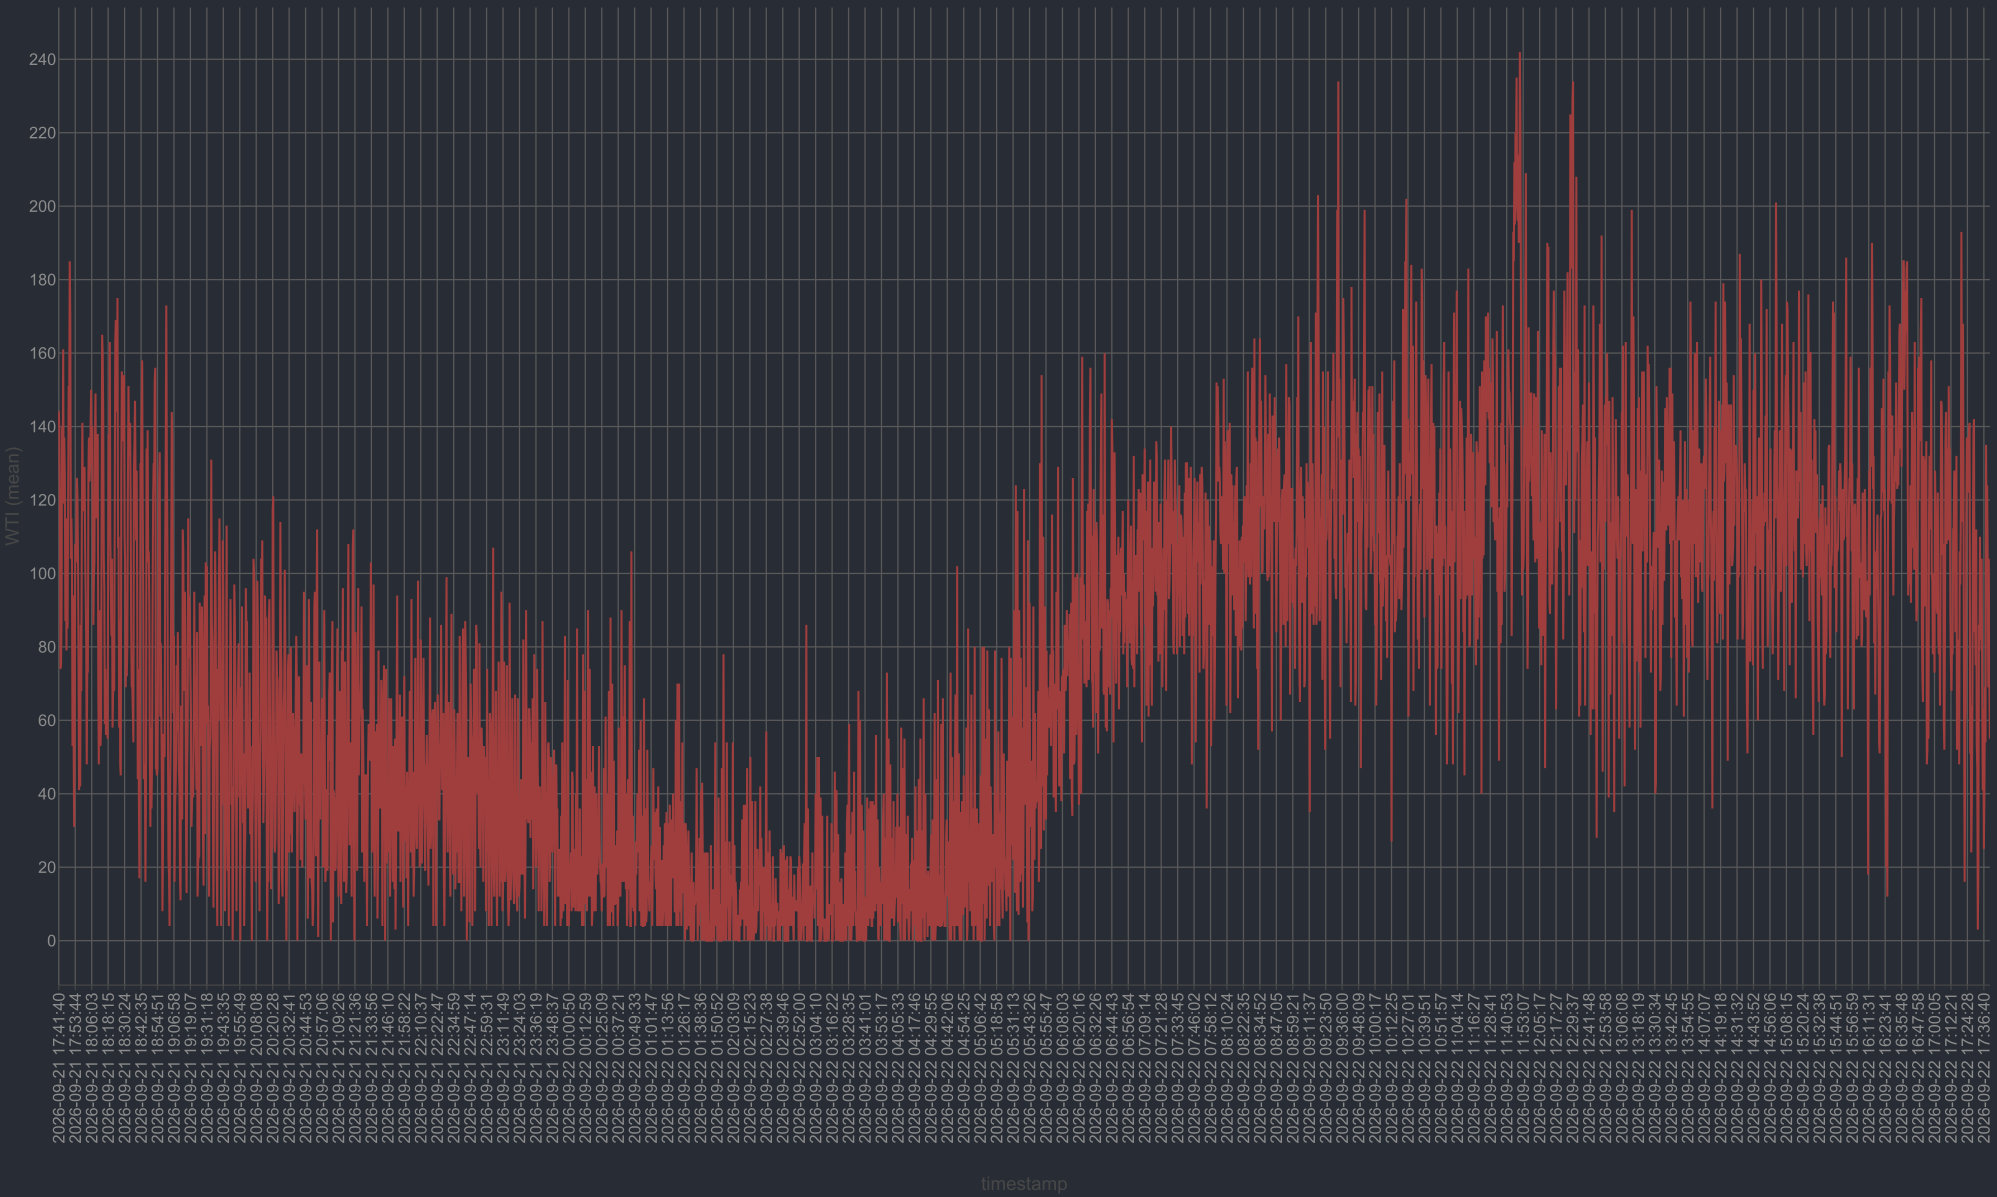
\includegraphics[width=\linewidth]{data/chart1.png}
        \caption{Biểu đồ WTI quan sát của đợt 21--22/09 (\texttt{data/chart1.png}). Vùng đêm có mức thấp, sau đó WTI tăng rõ khi chuyển sang buổi sáng.}
        \label{fig:chart1}
    \end{subfigure}
    \hfill
    \begin{subfigure}[t]{0.48\textwidth}
        \centering
        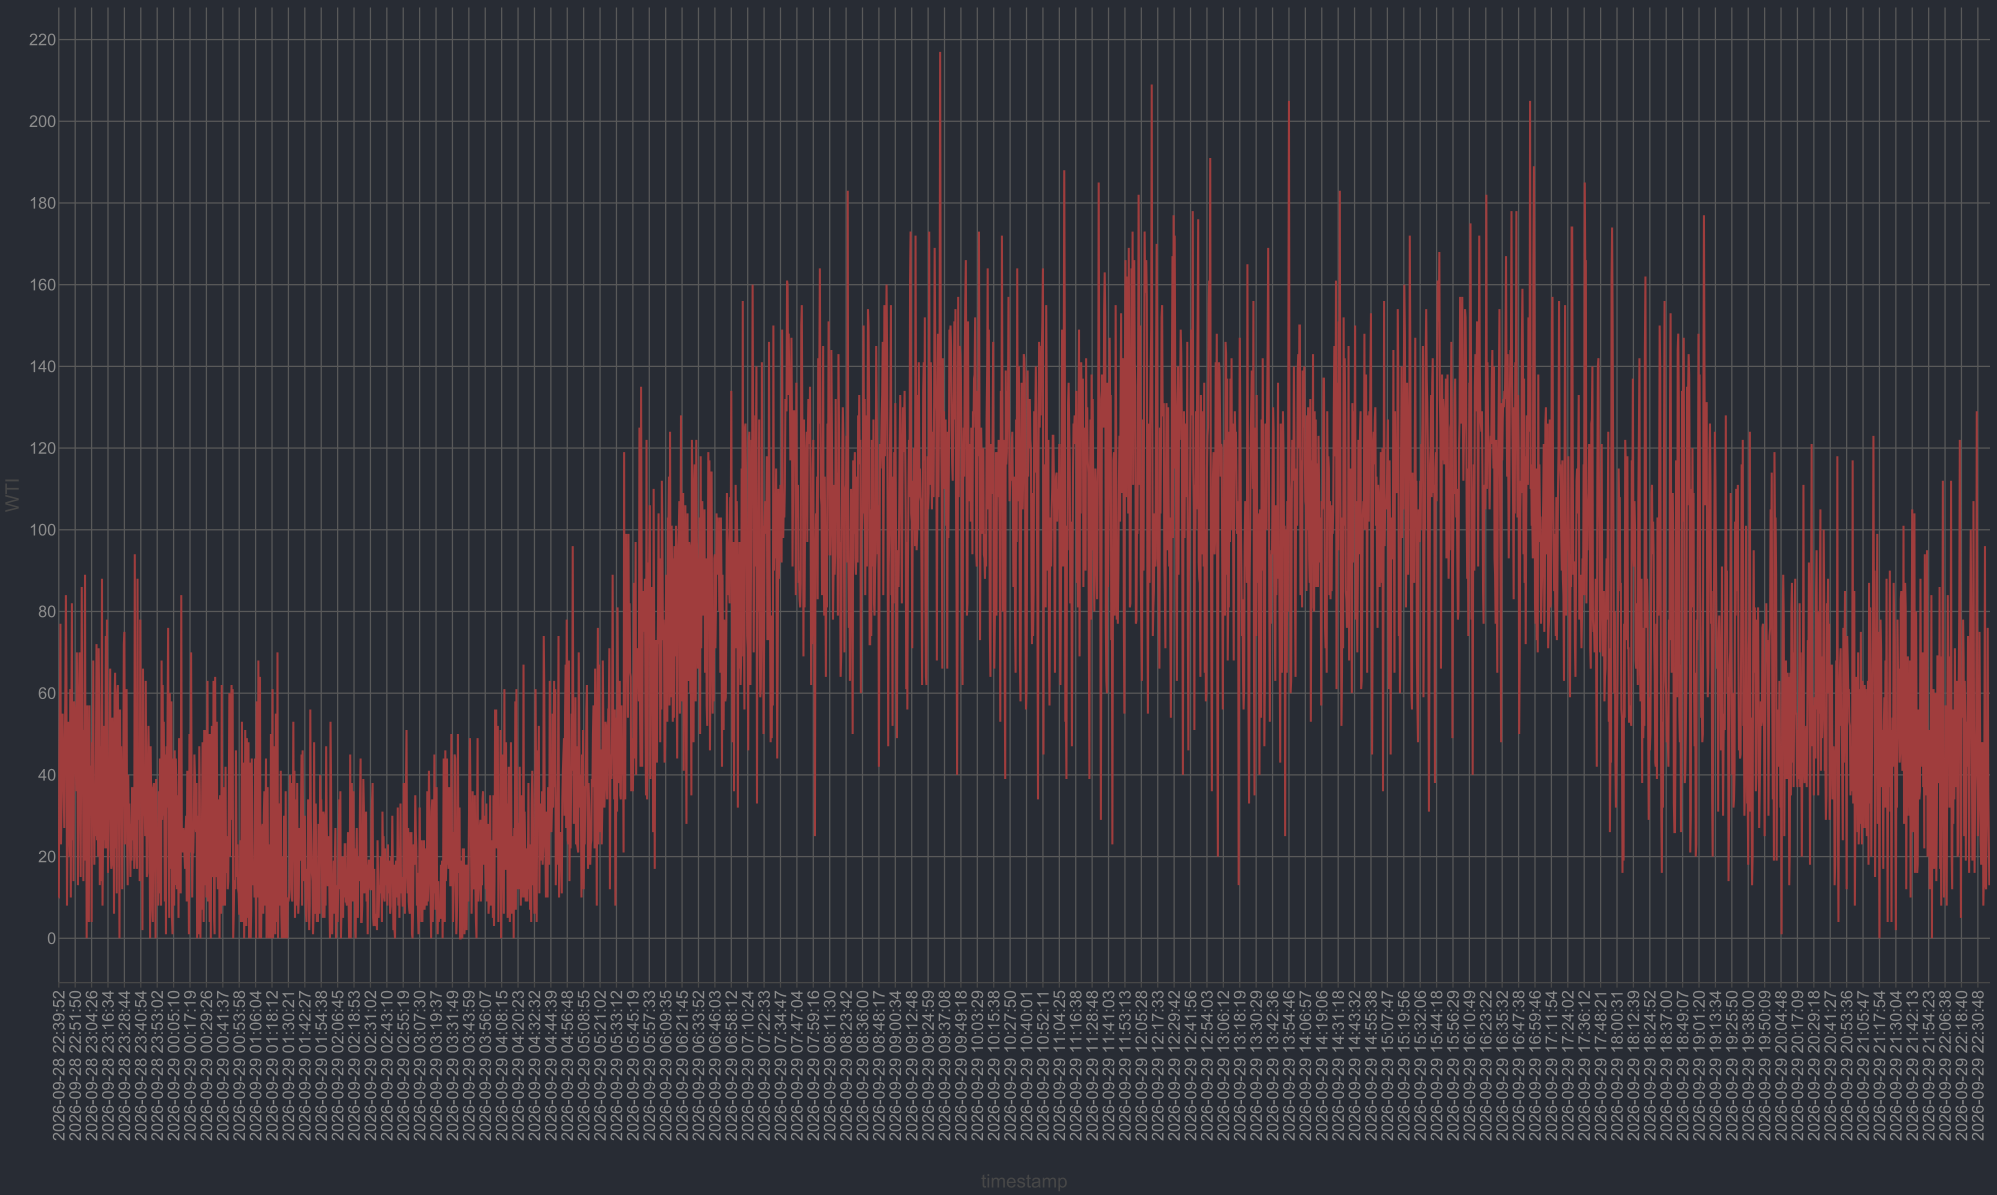
\includegraphics[width=\linewidth]{data/chart2.png}
        \caption{Biểu đồ WTI quan sát của đợt 28--29/09 (\texttt{data/chart2.png}). Hai hình là biểu đồ dữ liệu đã thu, không phải kết quả dự báo.}
        \label{fig:chart2}
    \end{subfigure}
    \caption{Đối chiếu biểu đồ WTI quan sát thực tế giữa hai đợt thu thập dữ liệu.}
    \label{fig:comparison_charts}
    \end{figure}

    Hai đợt đều có WTI trung bình thấp vào khoảng 02 giờ. Tính trên chuỗi phút hoàn tất, giờ có WTI trung bình cao nhất là 11 giờ ở \texttt{data1} và 16 giờ ở \texttt{data2}. Điều này cho thấy vị trí đỉnh và hình dạng chuỗi có thay đổi giữa các đợt; không nên coi một ngày tham chiếu là quy luật cố định. Đỉnh WTI cũng không nhất thiết trùng đỉnh tổng số xe vì thành phần phương tiện có trọng số khác nhau.

    \begin{figure}[htbp]
\centering
\begin{tikzpicture}
    % Định nghĩa 2 màu đặc trưng giống biểu đồ gốc
    \definecolor{colorData1}{RGB}{14, 124, 134} % Xanh teal
    \definecolor{colorData2}{RGB}{217, 119, 36}  % Cam đất

    \begin{axis}[
        title={\textbf{Đối chiếu nhịp ngày của hai đợt thu}},
        title style={font=\normalsize, yshift=2pt},
        width=0.92\textwidth,
        height=6.2cm,
        xlabel={Giờ trong ngày},
        ylabel={WTI trung bình},
        xlabel style={font=\small},
        ylabel style={font=\small},
        tick label style={font=\footnotesize},
        xmin=-0.8, xmax=23.8,
        ymin=7, ymax=138,
        xtick={0,2,4,6,8,10,12,14,16,18,20,22},
        ytick={20,40,60,80,100,120},
        % Cấu hình lưới mờ và trục tọa độ
        grid=both,
        grid style={line width=0.2pt, draw=gray!15},
        axis x line*=bottom,
        axis y line*=left,
        legend style={
            at={(0.97,0.95)},
            anchor=north east,
            draw=gray!30,
            fill=white,
            font=\footnotesize,
            cells={anchor=west}
        }
    ]

        % Đường biểu diễn data1 (Xanh teal)
        \addplot[
            color=colorData1,
            mark=*,
            mark size=1.8pt,
            line width=1.1pt
        ] coordinates {
            (0, 26.5) (1, 16.7) (2, 12.5) (3, 14.8) (4, 19.8) 
            (5, 38.9) (6, 85.0) (7, 99.0) (8, 110.5) (9, 118.2) 
            (10, 114.5) (11, 132.0) (12, 122.3) (13, 109.8) (14, 114.6) 
            (15, 116.8) (16, 115.5) (17, 97.0) (18, 97.5) (19, 60.9) 
            (20, 50.6) (21, 46.7) (22, 43.2) (23, 35.5)
        };
        \addlegendentry{data1}

        % Đường biểu diễn data2 (Cam đất)
        \addplot[
            color=colorData2,
            mark=*,
            mark size=1.8pt,
            line width=1.1pt
        ] coordinates {
            (0, 26.5) (1, 19.0) (2, 16.6) (3, 18.0) (4, 27.2) 
            (5, 52.0) (6, 79.6) (7, 99.5) (8, 106.3) (9, 115.0) 
            (10, 110.4) (11, 109.2) (12, 112.1) (13, 101.5) (14, 106.9) 
            (15, 108.3) (16, 120.0) (17, 99.0) (18, 80.7) (19, 69.6) 
            (20, 53.5) (21, 50.1) (22, 45.6) (23, 34.4)
        };
        \addlegendentry{data2}

    \end{axis}
\end{tikzpicture}
\caption{Đối chiếu biến thiên chỉ số WTI trung bình theo các khung giờ trong ngày giữa data1 và data2.}
\label{fig:hourly_wti_comparison}
\end{figure}
    \subsection{Chất lượng và tính đại diện}
    Kiểm tra trực tiếp cho thấy hai CSV không có ô trống hoặc timestamp trùng. Hàm kiểm tra của dự án chấp nhận toàn bộ bản ghi về số đếm nguyên không âm, giá trị hữu hạn và tính nhất quán của \texttt{total}, WTI. Mã băm SHA-256 của hai CSV hiện tại khớp thông tin dữ liệu trong báo cáo huấn luyện đã lưu.

    Tuy vậy, dữ liệu sạch ở cấp dòng vẫn có thể thiếu theo thời gian: 5 phút hoàn toàn vắng mẫu chỉ xuất hiện rõ sau khi đưa dữ liệu về lưới một phút. Ngoài ra, dữ liệu chưa có \texttt{camera\_id}, phiên bản detector, ROI, nhãn thời tiết, tốc độ hoặc nhãn ùn tắc. Hai đợt gần 24 giờ chưa đủ để đánh giá mùa vụ tuần, ngày lễ, sự cố hay khả năng chuyển sang giao lộ khác.

